\documentclass[a4paper, margin=1inch]{article}
\usepackage[margin=35mm]{geometry}

\synctex=1
\pdfoutput=1 

\usepackage[utf8]{inputenc}
\usepackage[T1]{fontenc}
\usepackage{lmodern}
\usepackage{microtype}

\usepackage[USenglish]{babel}

\usepackage{graphicx} % Required for inserting images
\usepackage{xcolor}
\usepackage{amsmath,amssymb,amsthm}
\usepackage[]{hyperref}
\hypersetup{
    colorlinks,
    linkcolor={red!50!black},
    citecolor={blue!50!black},
    urlcolor=.
}
\usepackage{float}
\usepackage[capitalize]{cleveref}
\usepackage{todonotes}
\usepackage{tabularx}
\usepackage[square,numbers]{natbib}
\usepackage{tikz}
\usetikzlibrary{calc}
\usetikzlibrary{positioning,backgrounds,patterns,calc,matrix,shapes,decorations.pathreplacing,decorations.pathmorphing,math}
\tikzset{crossing/.style={cross out, draw=red, minimum size=2*(#1-\pgflinewidth), inner sep=0pt, outer sep=1pt, very thick}, crossing/.default={4pt}}
\usetikzlibrary{arrows.meta,bending,decorations.markings,hobby,patterns,calc}
\newcolumntype{C}[1]{>{\centering\let\newline\\\arraybackslash\hspace{0pt}}m{#1}}

\usepackage{thmtools, thm-restate}
\newtheorem{redrule}{Reduction rule}
\newtheorem{claim}{Claim}
\newtheorem{lemma}{Lemma}
\newtheorem{corollary}{Corollary}
\newtheorem{observation}{Observation}
\newtheorem{proposition}{Proposition}
\newtheorem{definition}{Definition}
\newtheorem{theorem}{Theorem}

% Algorithms
\usepackage[ruled, vlined, linesnumbered, nofillcomment]{algorithm2e}
% taken from https://tex.stackexchange.com/questions/162207/algorithm2e-comment-style
\newcommand\commentstyle[1]{\footnotesize\ttfamily\textcolor{blue}{#1}}
\DontPrintSemicolon
\SetKwInOut{Input}{Input}
\SetKwInOut{Output}{Output}
\SetKwProg{Procedure}{Procedure}{}{}

%%%%%%%%%%%%%%%%%%%%%%%%%%%%%%%%%%%%%%%%%%%%%%%%%%%%%%
\newtheorem{assumption}{Assumption}
\newcommand{\cclass} [1] {\textnormal{\textsf{#1}}}

\usepackage{graphicx}
\usepackage{wrapfig}
\graphicspath{ {./figs/} }

\newcommand{\problemdef}[3]{
	\begin{center}
	\begin{minipage}{0.95\columnwidth}
		\noindent
		\textsc{#1}
		\vspace{5pt}\\
		\setlength{\tabcolsep}{3pt}
		\begin{tabularx}{\textwidth}{@{}lX@{}}
			\textbf{Input:}     & #2 \\
			\textbf{Question:}  & #3
		\end{tabularx}
	\end{minipage}
	\end{center}
}
\newcommand{\optproblemdef}[3]{
	\begin{center}
	\begin{minipage}{0.95\columnwidth}
		\noindent
		#1
		\vspace{5pt}\\
		\setlength{\tabcolsep}{3pt}
		\begin{tabularx}{\textwidth}{@{}lX@{}}
			\textbf{Input:}     & #2 \\
			\textbf{Task:}  & #3
		\end{tabularx}
	\end{minipage}
	\end{center}
}

\newcommand{\boxproblem}[4]{
    \begin{center}   
        \fbox{~\begin{minipage}{.97\textwidth}
            \vspace{2pt} 
            \noindent
            \normalsize\textsc{#1}
            \vspace{1pt}

            \setlength{\tabcolsep}{3pt}
            \renewcommand{\arraystretch}{1.0}
            \begin{tabularx}{\textwidth}{@{}lX@{}}
                \normalsize\textbf{Input:}       & \normalsize#2 \\
                \normalsize\textbf{Question:}    & \normalsize#3 \\
                \normalsize\textbf{Parameter: }  & \normalsize#4
            \end{tabularx}
        \end{minipage}}
    \end{center}
}
%%%%%%%%%%%%%%%%%%%%%%%%%%%%%%%%%%%%%%%%%%%%%%%%%%%%%%
\usepackage{authblk}
\newcommand{\email}[1]{ \href{mailto:#1}{\texttt{{#1}}}}

\newcommand{\MVVG}{\textsc{Maximum Value Vertex Guard}}
\newcommand{\MLVG}{\textsc{Maximum Length Vertex Guard}}
\newcommand{\DMVVG}{\textsc{Dynamic Maximum Value Vertex Guard}}
\newcommand{\BMVVG}{\textsc{Budgeted Maximum Value Vertex Guard}}



\title{Maximizing the Guarded Boundary of a Dynamic Art Gallery}
%\date{}

\author{Mihir Patel}



%%%%%%%%%%%%%%%%%%%%%%%%%%%%%%%%%%%%%%%%%%%%%%%%%%%%%%
\begin{document}

\maketitle

%mandatory: add short abstract of the document
\begin{abstract}
    An abstract.
\end{abstract}

% short version main body
\section{Introduction}
We consider a variant of the classic Art Gallery problem, where we instead seek to optimize the length of the boundary seen by the guards, not the number of guards themselves. Specifically, given a simple polygon $P$ and $k\in\mathbb{N}$, we want to find the $k$ vertex guards which maximize the length of the boundary of $P$ that is watched. We define the set of vertices of $P$ as $V_P$, and $L(S)$ as the length of the boundary seen by the set of vertex guards/vertices $S$. Note that $L(S)$ is necessarily at most the perimeter of $P$. 

\optproblemdef{\MLVG}{A simple polygon $P$ and a positive integer $k\in\mathbb{N}$.}{Find a set of vertices $S\subseteq V_P$ of size at most $k$ such that $L(S)$ is maximized.}

We also consider a weighted variant of this problem, where $P$ is a simple polygon composed of (possibly collinear) weighted line segments. Art galleries contain paintings, and some have more value than others. With limited guards, a realistic task would be to maximize not the total boundary watched, but the total value of paintings watched. In our definition, a weighted segment must be completely seen by our $k$ guards to be considered ``watched''. We define $W(S)$ as the weighted analog of $L(S)$, the sum of weights of all segments on the boundary of $P$ that are completely watched by guards in $S$.

\optproblemdef{\MVVG}{A weighted polygon $P$ and a positive integer $k\in\mathbb{N}$.}{Find a set of vertices $S\subseteq V_P$ of size at most $k$ such that $W(S)$ is maximized.}

Finally, we consider a dynamic version of \MVVG, which we'll call \DMVVG. New paintings may arrive in an art gallery, and their arrangement around the gallery may change. Thinking of vertex guards as cameras, it can be costly and time-consuming rearrange and reinstall cameras across the room (at least compared to moving the paintings around). If the segment weights on the weighted polygon change, how can we modify our solution (with minimal changes) to maintain an approximate solution for \MVVG\ at each timestep?
\todo[inline]{Obviously this dynamic problem needs to be specified a lot more, but hopefully the general idea of/motivation for the problem is showing through. I am trying to create a dynamic set cover analog for art gallery, where elements are inserted/removed one at a time, and the goal is to maintain a set cover that is still an approximate solution (without simply recalculating a set cover at each change).}


\subsection{Related Works}
\todo[inline]{Need a paragraph discussing more conventional Art gallery problem literature (authors+results). Klee, O'Rourke, Das}
In \cite{fragoudakis-interior,fragoudakis-boundary,fragoudakis-paintings}, Fragoudakis et al. pose both \MLVG\ and \MVVG. They prove that both problems are APX-complete in \cite{fragoudakis-boundary}, meaning these problems are NP-hard and also permit no PTAS unless $P=NP$. In \cite{fragoudakis-interior}, they present a $(1-1/e)$-approximation for maximizing the vertex-guarded \emph{interior} of a polygon which runs in $O(k^2n^2)$ and depends on segmenting the polygon into visibility regions.

\cite{abdelkader} presents several inapproximability results for art gallery problems, with $\alpha$-Floodlights.

\todo[inline]{Need to discuss some more dynamic set cover. Here is the most recent paper I've been able to find.}

\cite{bukov}

\subsection{Our Contributions}
For \MLVG\ and \MVVG, we extend the results from \cite{fragoudakis-interior} to get a $(1-1/e)$-approximation, that runs in $O(kn^2)$. We use the monotonicity and submodularity of our objective functions $L$ and $W$ to get this bound, presenting a simpler (and slightly more efficient) approach than the Finest Visbility Segmentation approach from \cite{fragoudakis-interior,fragoudakis-paintings}. We also prove several inapproximability results for these problems.

For \DMVVG, we analyze the performance of several strategies, showing some of them may perform arbitrarily badly compared to an optimal solution, while some achieve a bound. 









\section{Submodularity of \MVVG{}}
In this section, we prove that the objective functions of both \MLVG{} and \MVVG{} are monotone and submodular. This then implies that greedily maximizing the objective will yield a $(1-\frac{1}{e})$ approximation for both problems. We also provide a brief analysis of the running time of these greedy algorithms, which is an improvement on the approximation algorithms proposed for these problems in \cite{fragoudakis-interior,fragoudakis-boundary,fragoudakis-paintings}.\\\\
We start with the objective function of \MLVG{}, $L$. Recall that given a simple polygon $P$ and a set of vertex guards $S\subseteq V_P$, $L(S)$ denotes the length of the guarded boundary of $P$, and is necessarily less than or equal to the permiter of $P$. It is fairly immediate to see that $L$ is monotone.

\begin{observation}\label{obs:monotone}
    For any $S\subseteq T\subseteq V$, $L(S)\leq L(T)$.
\end{observation}

\begin{proof}
    Consider a point $p$ on the portion of the boundary of the polygon counted by $L(S)$, then $p$ must be seen by some $v\in S$. As $S\subseteq T$, $v\in T$ as well, implying $p$ is counted by $L(T)$. Every point on the boundary counted by $L(S)$ is also counted by $L(T)$, and thus $L(S)\leq L(T)$. 
\end{proof}
\noindent
We can also show that $L$ is submodular with a little bit more work.

\begin{claim}\label{clm:submodular}
    For any $S\subseteq T\subseteq V$ and $v\notin T$, $L(S\cup\{v\})-L(S)\geq L(T\cup\{v\})-L(T)$.
\end{claim}

\begin{proof}
    First observe that, by~\Cref{obs:monotone}, $L(S\cup\{v\})-L(S)\geq 0$, meaning this claim is trivial if $L(T\cup\{v\})-L(T)\leq 0$. So we only consider the case where $L(T\cup\{v\})-L(T)>0$, or in other words, there is some portion of the boundary of the polygon guarded by $T\cup\{v\}$, but not $T$. Then for every point $p$ in this portion, $p$ is visible to $v$, but not $T$. As $S\subseteq T$, by~\Cref{obs:monotone}, $p$ is visible to $S$ either. \\\\
    In short, we know that $p$ is visible to $S\cup\{v\}$ but not $S$, and as this is true for every point on the boundary seen by the set of guards $T\cup\{v\}$, but not $T$, $L(S\cup\{v\})-L(S)\geq L(T\cup\{v\})-L(T)$, as desired.
\end{proof}
\noindent
These two facts also lift quickly to the objective function of \MVVG{}, $W$. Given a simple polygon $P$ made up of weighted segments and a set of vertex guards $S\subseteq V_P$, $W(S)$ denotes the total weight of the guarded boundary of $P$. Note that a weighted segment must be \emph{completely} visible to a set of guards to be considered ``guarded'' and contribute to the total weight. The proofs of monotonicity and submodularity for $W$ proceed exactly the same as those of $L$ (we only need to swap $L$ and $W$).

\begin{observation}\label{obs:monotone-w}
    For any $S\subseteq T\subseteq V$, $W(S)\leq W(T)$.
\end{observation}

\begin{claim}\label{clm:submodular-w}
    For any $S\subseteq T\subseteq V$ and $v\notin T$, $W(S\cup\{v\})-W(S)\geq W(T\cup\{v\})-W(T)$.
\end{claim}
\noindent
Equipped with these properties of $L$ and $W$, we can quickly derive greedy algorithms for \MLVG{} and \MVVG{}. Start with an empty solution set $S$. While the size of $S$ is less than $k$, find the vertex $v$ which provides $L$ with the most marginal gain. That is, the vertex $v$ which maximizes $L(S\cup\{v\})-L(S)$. Then add $v$ to $S$ and repeat, until $|S|=k$. Then, because $L$ and $W$ are both monotone submodular, we get the following facts about maximizing monotone submodular functions under cardinality constraints (i.e. the type of problem \MLVG{} and \MVVG{} both are).

\begin{theorem}[\cite{cornuejols}]
    The greedy algorithm is a $(1-1/e)$-approximation algorithm for \MLVG{}. 
\end{theorem}

\begin{theorem}[\cite{feige}]
    For any $\epsilon>0$, there is no $(1-1/e+\epsilon)$-approximation algorithm for \MLVG{}, unless \cclass{P}=\cclass{NP}.
\end{theorem}
\noindent
The same approximation guarantees hold for the greedy algorithm applied to \MVVG{}, which maximizes the marginal gain of $W$. As for the runtime of these algorithms, they proceed in $k$ iterations, selecting one vertex per step. In each iteration, we evaluate the marginal gain for up to $n$ candidate vertices. To compute the marginal gain of a vertex $v$, we maintain the portion of the boundary currently guarded by the selected set $S$, compute the portion guarded by $v$, and take their union to determine the new coverage. Since computing the visibility region of a single vertex can be done in $O(n)$ time \cite{visibility}, and union operations can be managed efficiently with appropriate data structures, each marginal gain evaluation takes $O(n)$. Thus, the total running time of the greedy algorithm is $O(kn^2)$ in the worst case.\\\\
By leveraging the monotonicity and submodularity of the objective functions in \MLVG{} and \MVVG{}, we obtain simple greedy algorithms that achieve a $(1-1/e)$-approximation. While previous work \cite{fragoudakis-boundary,fragoudakis-interior,fragoudakis-paintings} also achieves this approximation ratio, we additionally prove that this is the best possible approximation ratio unless \cclass{P}=\cclass{NP}. Moreover, our approach offers a slight improvement in efficiency: our algorithms run in $O(kn^2)$ time, whereas their algorithms have runtimes of $O(n^4)$ and $O(k^2n^2)$.
\section{Intuition-Building Examples for \BMVVG{}}
In this section, we show that three natural greedy strategies for \BMVVG{} may all perform arbitrarily badly compared to an optimal solution. In other words, these strategies will not automatically form approximations for \BMVVG{}, as there exists a problem instance where the total weight they achieve is \emph{not} boundedly close to the optimal. Note that this is in contrast to \MLVG{} and \MVVG{}, where the natural greedy strategy formed a constant-factor approximation, validating the added difficulty of \BMVVG{}. \\\\
A first attempt could be to greedily add the vertex which maximizes the total weight guarded. To see why this fails, fix a $w\in\mathbb{N}$ such that $w\geq 3$. Then construct the polygon depicted in~\Cref{fig:greedy-heaviest}, with $w$ many ``cones''. The right edge of each cone has weight $w$, while all other edges have weight 1. The apex of each cone has cost $w$, while all other vertices have cost $w^2$. The budget $B$ is equal to $w^2$, and now we have an instance of \BMVVG{}, with~\Cref{fig:greedy-heaviest} and $B=w^2$.
\begin{figure}
    \centering
    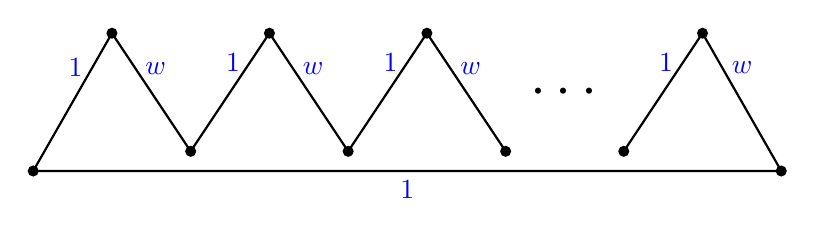
\begin{tikzpicture}
        %cone 1
        \coordinate (a) at (0, -.25);
        \coordinate (b) at (1, 1.5);
        \coordinate (c) at (2, 0);
        %cone 2
        \coordinate (d) at (3, 1.5);
        \coordinate (e) at (4, 0);
        %cone 3
        \coordinate (f) at (5, 1.5);
        \coordinate (g) at (6, 0);

        %cone 4
        \coordinate (h) at (7.5, 0);
        \coordinate (i) at (8.5, 1.5);
        \coordinate (j) at (9.5, -.25);

        % Draw the polygon
        \draw[thick] (a) -- (b) -- (c) -- (d) -- (e) -- (f) -- (g);
        \draw[thick] (h) -- (i) -- (j) -- (a);

        % Add dots at each vertex
        \fill (a) circle (2pt);
        \fill (b) circle (2pt);
        \fill (c) circle (2pt);
        \fill (d) circle (2pt);
        \fill (e) circle (2pt);
        \fill (f) circle (2pt);
        \fill (g) circle (2pt);
        \fill (h) circle (2pt);
        \fill (i) circle (2pt);
        \fill (j) circle (2pt);

        %ellipsis
        \node at (6.8, .75) {\huge$\cdots$};

        % Add edge weights 
        \node[left, text=blue] at ($(a)!0.75!(b)$) {$1$};
        \node[right, text=blue] at ($(b)!0.3!(c)$) {$w$};

        \node[left, text=blue] at ($(c)!0.75!(d)$) {$1$};
        \node[right, text=blue] at ($(d)!0.3!(e)$) {$w$};

        \node[left, text=blue] at ($(e)!0.75!(f)$) {$1$};
        \node[right, text=blue] at ($(f)!0.3!(g)$) {$w$};

        \node[left, text=blue] at ($(h)!0.75!(i)$) {$1$};
        \node[right, text=blue] at ($(i)!0.25!(j)$) {$w$};

        \node[below, text=blue] at ($(a)!0.5!(j)$) {$1$};

    \end{tikzpicture}
    \caption{apex vertices have cost w, everything else has $w^2$, budget is $w^2$.}
    \label{fig:greedy-heaviest}
\end{figure}\\\\
Now the greedy strategy would start by choosing the vertex that maximizes the total weight guarded. Initially, this is one of the ``valleys'' in polygon, as these vertices guard $2w+2$ total weight, whereas all other vertices guard at most $w+1$. Any one of these vertices has cost $w^2$, so adding it to our solution uses our entire budget. Thus the algorithm which greedily maximizes total weight guarded ends up guarding $2w+2$ total weight on~\Cref{fig:greedy-heaviest}.\\\\
However, an optimal strategy would be to place a guard at each apex. There are $w$ many apices and each one has cost $w$, so to use all of them would cost $w^2$ (which is exactly our budget). This guard placement also guards our entire polygon boundary, meaning the total weight guarded by the optimal set of guards is $w(w)+w(1)+1=w^2+w+1$. To compare total weight achieved between these two algorithms, the weight achieved by the greedy divided by the weight achieved by the optimal is equal to $\frac{2w+2}{w^2+w+1}$. We can make this value arbitrarily small as we increase $w$, meaning the greedy algorithm which maximizes total weight guarded performs arbitrarily badly compared to an optimal solution.\\\\
Now we consider two alternative greedy strategies and show that they also fail, using~\Cref{fig:greedy-cheapest}. The first would be to greedily add the vertex with cheapest cost. The second would be to greedily add the vertex which maximizes the ratio of marginal gain in total weight to vertex cost. Starting with the first strategy, consider~\Cref{fig:greedy-cheapest} where weights and costs are displayed, and the budget is $w+4$. The cheapest vertex is $A$, which has cost of $2$. The vertex $A$ guards total weight of $2$, and once we have placed a guard there we cannot afford to place guards at any of the remaining vertices. Thus this greedy choosing the cheapest vertex achieves total weight of $2$ on this example. An optimal strategy would be to place a guard on either $D$ or $B$, this stays within budget and guards the entire polygon, achieving total weight of $w+3$. Comparing the weight achieved by each strategy, we have $\frac{2}{w+3}$, which we can make arbitrarily small as we increase $w$.
\begin{figure}
    \centering
    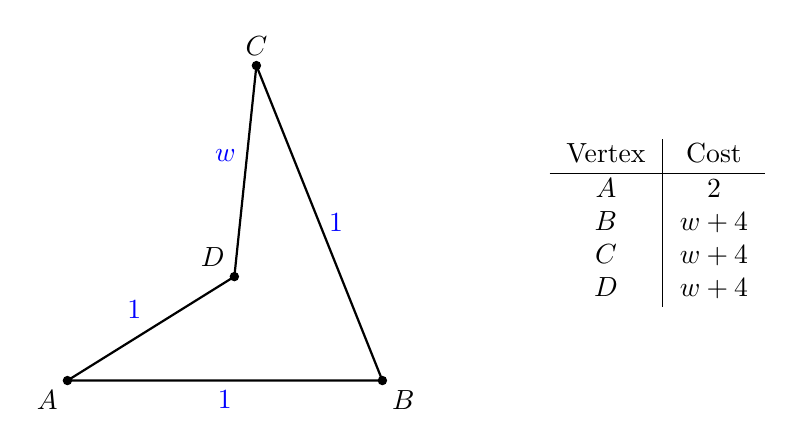
\begin{tikzpicture}[scale=4]
        % Define the points of the reflex quadrilateral
        \coordinate (A) at (0, 0);
        \coordinate (B) at (1, 0);
        \coordinate (C) at (0.6, 1);
        \coordinate (D) at (.53, .33); % Reflex angle at D

        % Draw the polygon
        \draw[thick] (A) -- (B) -- (C) -- (D) -- cycle;

        % Draw vertex dots
        \foreach \point in {A,B,C,D}
            \fill (\point) circle (0.015);

        % Label the vertices
        \node[below left] at (A) {$A$};
        \node[below right] at (B) {$B$};
        \node[above] at (C) {$C$};
        \node[above left] at (D) {$D$};

        % Add edge weights (all same color)
        \node[below, text=blue] at ($(A)!0.5!(B)$) {$1$};
        \node[right, text=blue] at ($(B)!0.5!(C)$) {$1$};
        \node[above left, text=blue] at ($(C)!0.5!(D)$) {$w$}; % edge with weight w
        \node[above left, text=blue] at ($(D)!0.5!(A)$) {$1$};

        % Compute average y-coordinate for alignment
        \path let \p1 = (A), \p2 = (C) in
            coordinate (tableanchor) at ($(0, {(\y1 + \y2)/2})$);

        % Add cost table to the right, vertically aligned with polygon
        \node[anchor=west] at ($(B) + (.5cm, 0.5cm)$) {
            \begin{tabular}{c|c}
            Vertex & Cost \\
            \hline
            $A$ & $2$ \\
            $B$ & $w + 4$ \\
            $C$ & $w + 4$ \\
            $D$ & $w + 4$ \\
            \end{tabular}
        };

    \end{tikzpicture}
    \caption{caption}
    \label{fig:greedy-cheapest}
\end{figure}\\\\
Similarly, if we wanted to greedily choose the vertex which maximizes the ratio of marginal gain in total weight to vertex cost (i.e., provides the best ``bang-for-your-buck''), we would choose vertex $A$. It guards weight of $2$ and costs $2$, giving a ratio of $1$. Any other vertex can guard at most $w+3$, while costing $w+4$, and $\frac{w+3}{w+4}<1$ for all $w$. Again, choosing $A$ prevents adding any more guards, achieving a total guarded weight of $2$, while an optimal strategy could guard $w+3$, and $\frac{2}{w+3}$ can be arbitrarily small for large $w$. \\\\
\cite{khuller} considers an analagous problem of covering as many elements as possible with sets, subject to a budget. They similarly show that greedily adding the set which maximizes the ratio of marginal gain in total weight to set cost does not form an approximation. However, they show that if you take the collection of sets $\mathcal{S}$ obtained by this greedy strategy, and you also take the single set which covers the most weight $S_t$, and then you output whichever one covers more weight, you get a $\frac{1}{2}(1-1/e)$-approximation for their problem. And they also show that this simple strategy can be further refined to obtain a $(1-1/e)$-approximation. A logical next step for \BMVVG{} would be to see how well these strategies can do. That is, if we take the set of vertices which was greedily chosen by maximizing the ratio of marginal gain in total weight guarded to vertex cost, and we take the vertex which guards the most weight alone, and we return whichever set of guards ends up guarding more weight, does this give us an approximation? Is it $\frac{1}{2}(1-1/e)$?





\section{Conclusion}


\bibliographystyle{abbrvnat}
\bibliography{refs}


\end{document}
